\section{Host directed anti‐viral strategies}

Currently available influenza drugs  target viral proteins M2 and NA. This approach allows for a specific mechanism of action, which, ideally, should not interfere with host cellular systems.

One significant problem with this approach is that, by introducing the antiviral drugs into the clinic, we exert evolutionary pressure on the virus. In turn, through the process of antigentic drift the virus may modify its target protein to escape inhibition by the drug, rendering the drug useless (e.g. adamantanes).

These concerns over antiviral drug resistance, and growing awareness of host proteins involvement in successful infection led to the emergence of a new drug development approach. Instead of targeting a viral protein, we try to target a host cell protein involved in viral infection. Thus, we can inhibit infection without subjecting the virus to direct selection.

\begin{figure}
\begin{center}
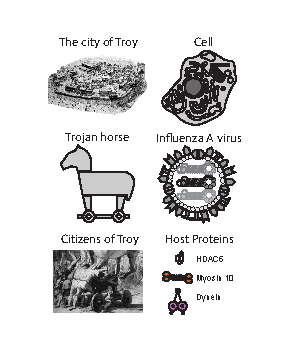
\includegraphics[width=0.7\textwidth, trim={0.6cm 0.6cm 0.6cm 0.6cm}, clip]{D_chapters/0_introduction/flu_troy.pdf}
\caption[Trojan siege metaphor for host directed anti-viral strategies]%
{Trojan siege metaphor for host directed anti-viral strategies. \par The city of Troy is a black and white render of reconstruction of the Homeric city of Troy, Turkey. (Photo by DeAgostini/Getty Images). The citizens of Troy are a black and white crop of "The Procession of the Trojan Horse into Troy from Two Sketches Depicting the Trojan Horse", oil on canvas by Giovanni Domenico Tiepolo, c. 1760 in the National Gallery, London.}
\label{figure:fluTroy}
\end{center}
\end{figure}

Conceptually such an approach can be understood through the story of a Trojan siege (Figure \ref{figure:fluTroy}). Much like a Trojan horse, which could not make it inside the city without the help of its citizens, viruses require host protein help for successful infection. Choosing to target these host proteins in an antiviral treatment is alike to convincing the Trojans to leave the horse at the door.

A major challenge in host directed anti‐viral strategies is cellular toxicity (which, however, is not exclusive to this approach). It is a complex issue, which we believe is best addressed by interrogating systemically the involvement of the protein in both cellular and viral processes, as well as elucidating the specific mechanism of action of a drug-like agent.